\documentclass[12pt]{article}
\usepackage{amsmath}
\usepackage{graphicx}
\usepackage{float}
\usepackage[font={small,it}]{caption}
\pagenumbering{arabic}

%\graphicspath{{./img/}{~/GitHub/sayboltm/PHY480/Project3/Report/img/}}
\graphicspath{{./img/}}

% This is a comment

\begin{document}
	\title{Project 3: Ordinary Differential Equations and the Solar System}
	\author{Michael Saybolt \\ Bjon Charlery}
	
%	\date{\today}
	\date{5/2/2017}
	\maketitle
	\pagebreak

\begin{abstract}
%This project explored solving differential equations, specifically \\linear second order equations, by using a couple of different methods \\ which include LU Decomposition, Gauss Forward and Backward Substitution : General algorithm
%
\begin{itemize}
	\item Develop code for simulating solar system
	\item Object orient for modularity
	\item Multiple solvers for ODE
		\begin{itemize}
		\item Euler method
		\item Velocity Verlet metho
		\end{itemize}
	\item Test as it is created to isolate bugs before they grow
\end{itemize}
\end{abstract}

\bigskip
\bigskip

\section{Introduction}
%\indent The objective of this project was to solve a differential equation in the form of:\\ $$-u\textsuperscript{''}(x) = f(x), x\epsilon(0,1),u(0) = u(1) = 0.\\$$ that can be written into the linear equation $(Ax = b)$. Since A is a tridiagonal matrix there is an actual or analytical solution that can be made for this particular matrix. The following sections will describe the origins for the algorithms used and their respective results.
%
\begin{itemize}
	\item For ease of debugging, a simulation of a simple binary system is created with just the Sun and the Earth
\end{itemize}
The only force in the problem is gravity. Newton's law of gravitation  is given by a force $F_G$
\[
F_G=\frac{GM_{\odot}M_{\mathrm{Earth}}}{r^2},
\]
where $M_{\odot}$ is the mass of the Sun and $M_{\mathrm{Earth}}$ is the mass of the Earth. The gravitational constant is $G$ and $r$ is the distance between the Earth and the Sun. Eventually the other planets will be added, but for now just this system will be used to test the layout of the algorithms.


\section{Description}
%This section will detail the methods used to solve the linear equation system. It is solved using two methods:\\
%\begin{itemize}
%	\item \centering LU decomposition
%	\item \centering Tridiagonal Solver - Gauss Elimination\\
%\end{itemize}
This section will provide details about the general equations describing the sytem, and the general approach of the problem.

\subsection{Block tied to wall}
Newton's equation of motion for system:
\[
m\frac{d^2x}{dt^2}=-kx,
\]
aka:
\[
\frac{d^2x}{dt^2}=-\frac{k}{m}x=-\omega_0^2x,
\label{eq:newton1}
\]
with the angular frequency $\omega_0^2=k/m$.

see line 1116 of ode.tex @Author: mhjensen for more equation

\subsection{Euler Method}
\begin{itemize}
	\item Euler
	\item Enhanced Euler
		\begin{itemize}
			\item Better numerical stability
		\end{itemize}
\end{itemize}

\subsection{Verlet Method}
\begin{itemize}
	\item Verlet
	\item Velocity Verlet
		\begin{itemize}
			\item Method with velocity is studied here
		\end{itemize}
\end{itemize}


\section{Implementation}
This section will transform the equations described in the previous section into usable code, and also describe difficulties encountered, and implemented solutions.

For 2D simplification, get 4 coupled DEs:
\[
	\frac{dv_x}{dt}=-\frac{GM_{\odot}}{r^3}x,
\]
\[
	\frac{dx}{dt}=v_x,
\]
\[
	\frac{dv_y}{dt}=-\frac{GM_{\odot}}{r^3}y,
\]
\[
	\frac{dy}{dt}=v_y
\]

This would be the same for 1 or 3 dimensions. But,
\[
	GM_{\odot}=v^2r,
	\]

and assuming Earth's velocity is:
$v = 2\pi r/\mathrm{yr}=2\pi\mathrm{AU}/\mathrm{yr}$

Thus can equate the following for the velocity in some direction:

\[
	\frac{dv_x}{dt} = -\frac{GM_{\odot}}{r^3}x = 4\pi^2 \frac{(\mathrm{AU})^3}{\mathrm{yr}^2}
\]

\subsection{Euler}
insert discretized

insert code

\subsubsection{Enhanced Euler}
\begin{itemize}
	\item better numerical stability as show in results
\end{itemize}

\subsection{Velocity Verlet}
\begin{itemize}
	\item As numerically stable as enhanced Euler
\end{itemize}











\section{Results}
%This section will show the overall correctness of each calculation, and the average speed of each method.
Results are presented here
\def \variable {my_var}=.75

\subsection{Euler}
%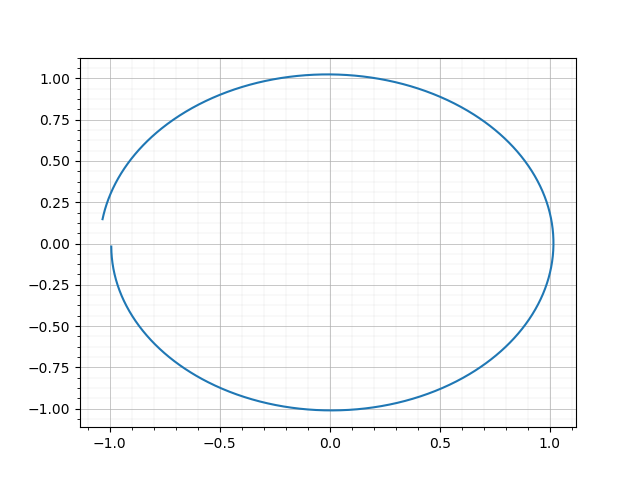
\includegraphics[scale=my_var]{binary_euler.png}
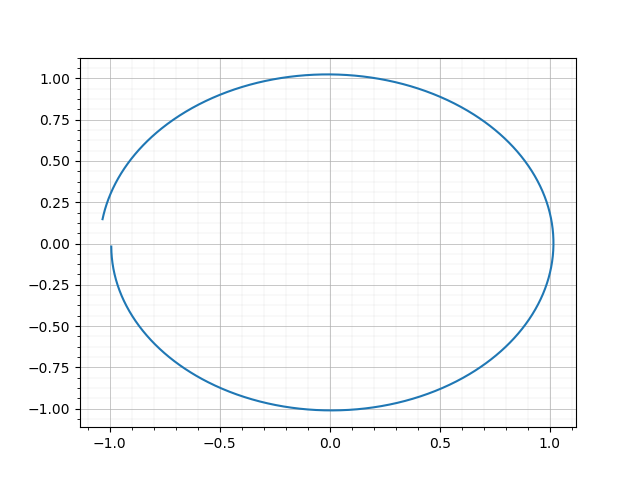
\includegraphics[scale=0.5]{binary_euler.png}

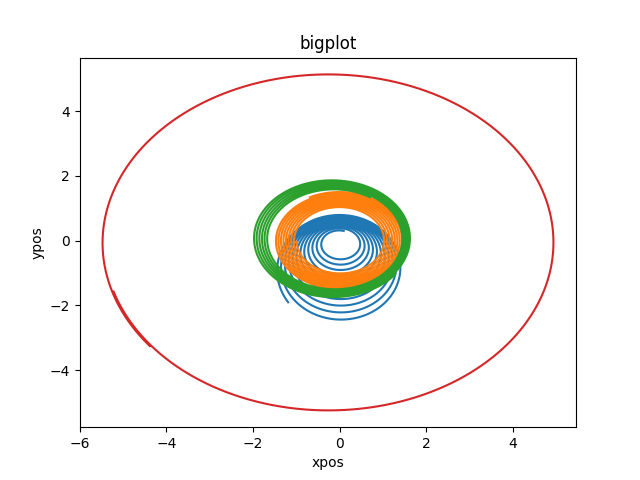
\includegraphics[scale=0.5]{euler_multiplanet.png}

\subsection{Enhanced Euler}
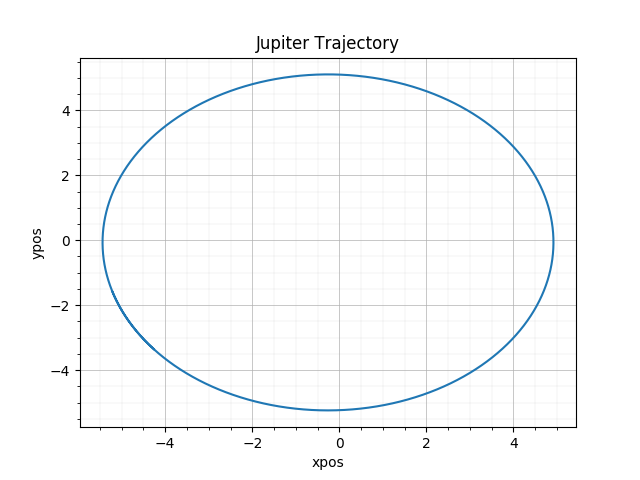
\includegraphics[scale=0.5]{euler_enhanced_jupiter.png}
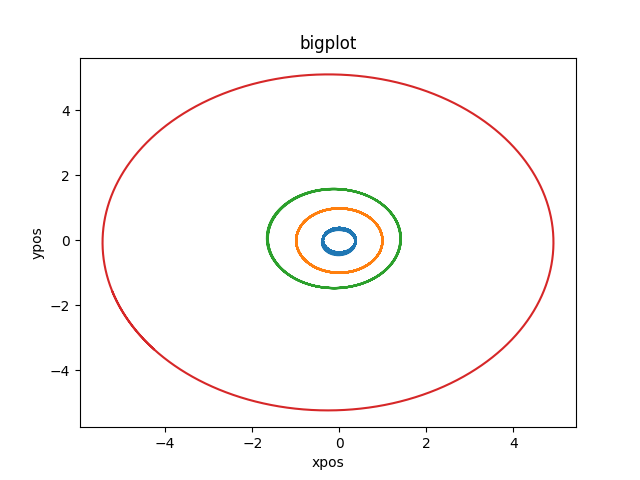
\includegraphics[scale=0.5]{euler_enhanced_multiplanet.png}

\subsection{Velocity Verlet}
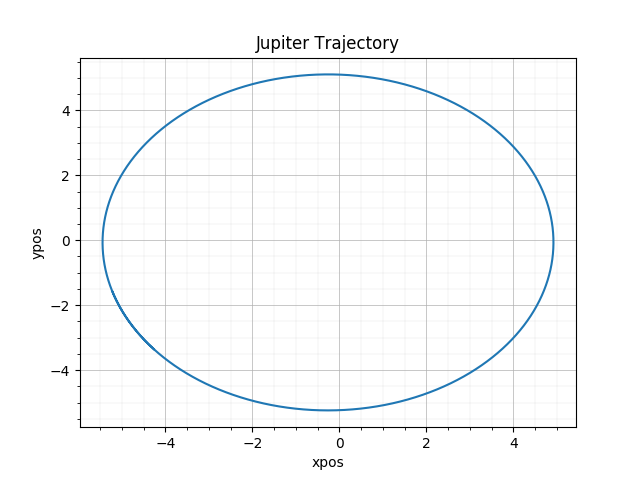
\includegraphics[scale=0.5]{verlet_jupiter.png}
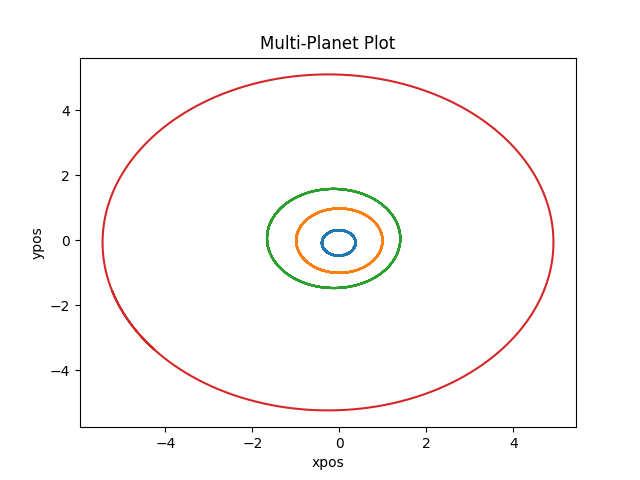
\includegraphics[scale=0.5]{verlet_multiplanet.png}

\subsection{Accuracy}
%The analytical solution to f(x) = 100*exp(-10*x) is known to be u(x) = 1-(1-exp(-10))*x-exp(-10*x). This is used to compare the accuracy of the numerical solutions obtained with both the general Gaussian elimination algorithm as well as the LU decomposition version for various n.  Plots are generated to give a summarized view of the generated output files.\\

\subsection{Gauss General:}
%Figure x shows the analytical solution and the numerical solution for various n using the general Gaussian elimination solver. As n increases, the result is more tightly fit to the analytical solution.\\
%
%\begin{figure}[H]
%\graphicspath{ {c:/Users/charl/Documents/Precision/Gauss/}{C:/Users/Mike/Documents/GitHub/sayboltm/PHY480/Project1/Report/Precision/Gauss/}}
%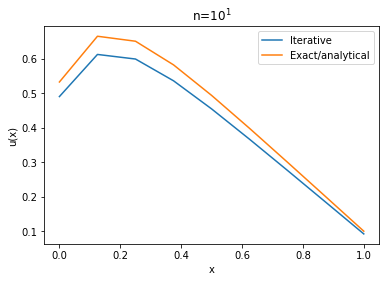
\includegraphics[scale=0.22]{1.png}
%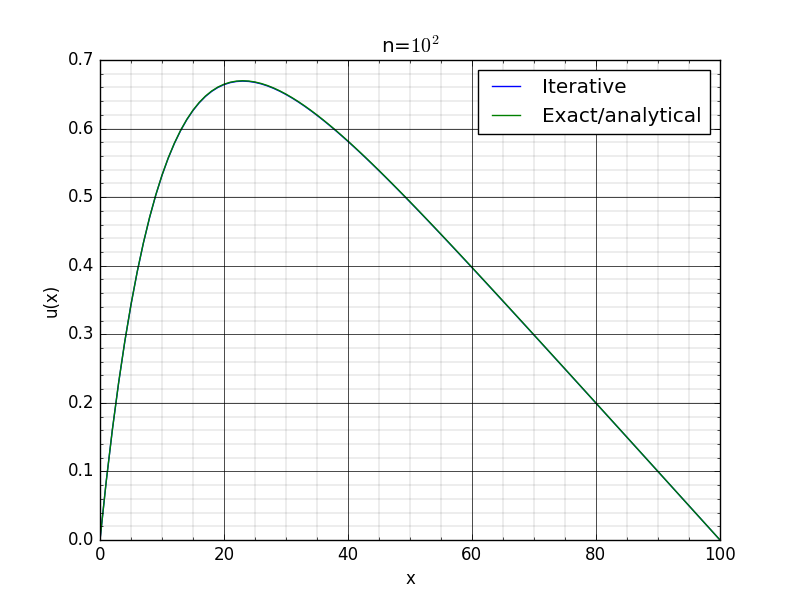
\includegraphics[scale=0.22]{2.png}
%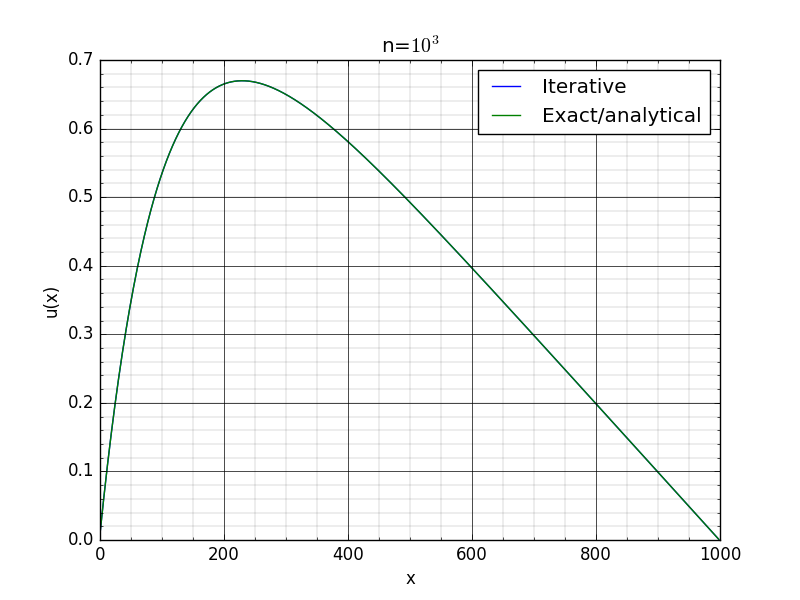
\includegraphics[scale=0.22]{3.png}
%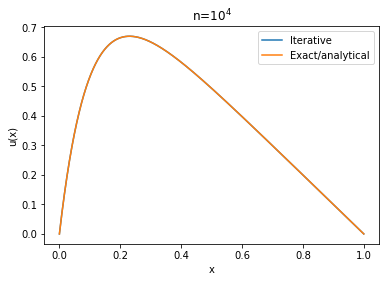
\includegraphics[scale=0.22]{4.png}
%\centering
%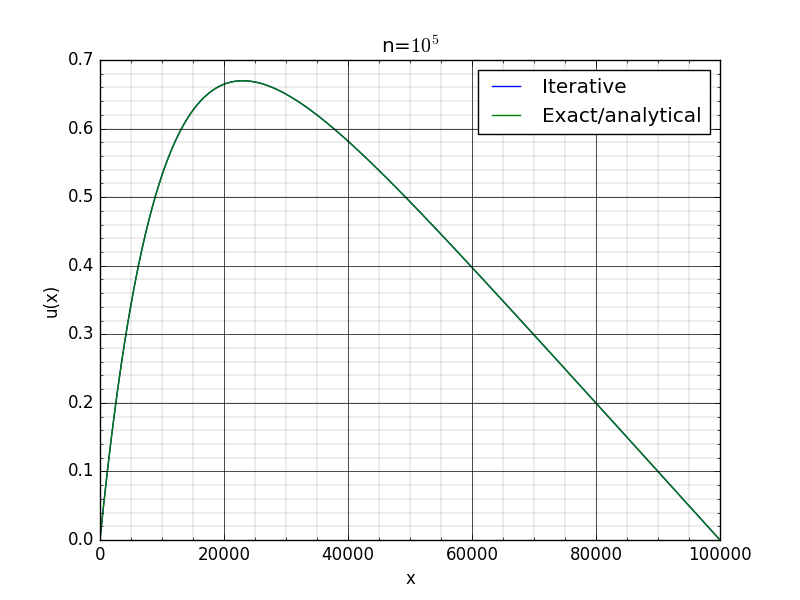
\includegraphics[scale=0.22]{5.png}\\
%\centering
%\caption{The relative error is computed using:
%	e\textsubscript{i}=|(v\textsubscript{i}-u\textsubscript{i})/(u\textsubscript{i})
%	where v\textsubscript{i} is the analytical solution value, and u\textsubscript{i} is the numerical solution value}
%\end{figure}
%The relative error is plotted for various n in figure y.\\
%\begin{figure}[H]
%\centering
%\graphicspath{ {c:/Users/charl/Documents/Precision/Gauss/}{C:/Users/Mike/Documents/GitHub/sayboltm/PHY480/Project1/Report/Precision/Gauss/}}
%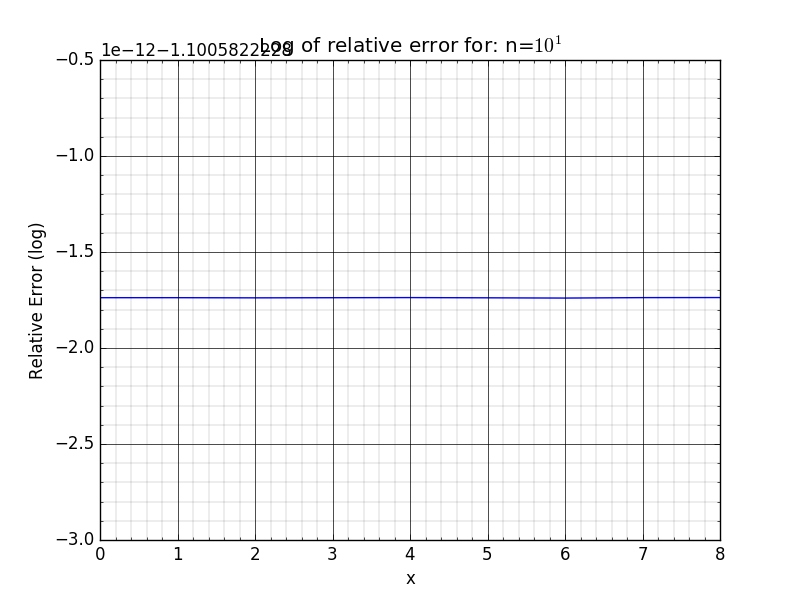
\includegraphics[scale=0.22]{1_error.png}
%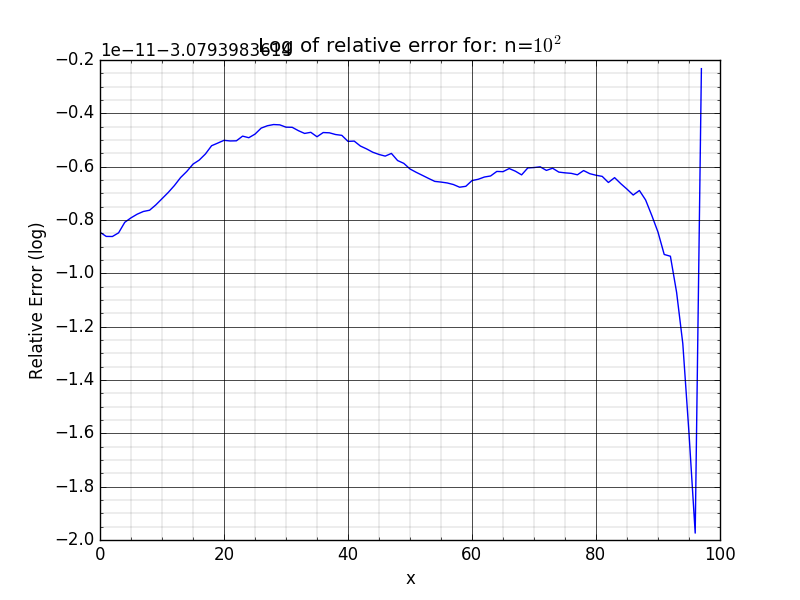
\includegraphics[scale=0.22]{2_error.png}
%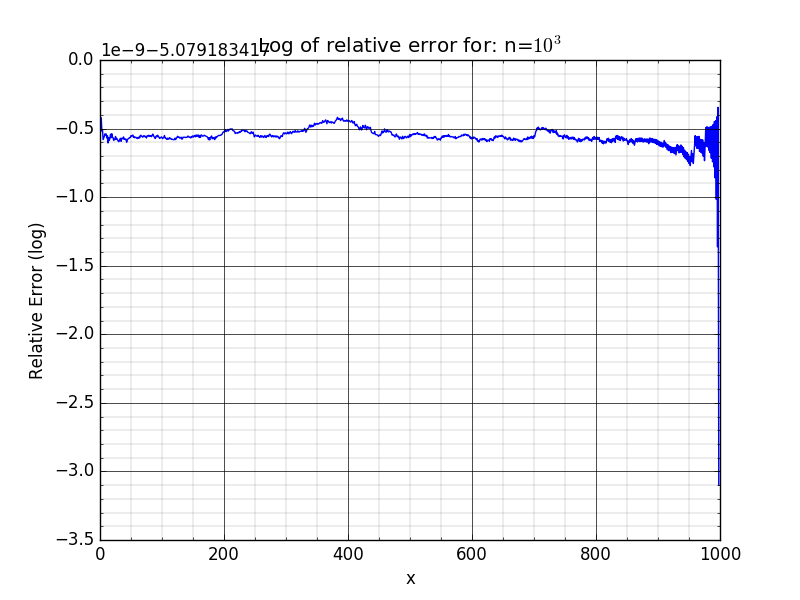
\includegraphics[scale=0.22]{3_error.png}
%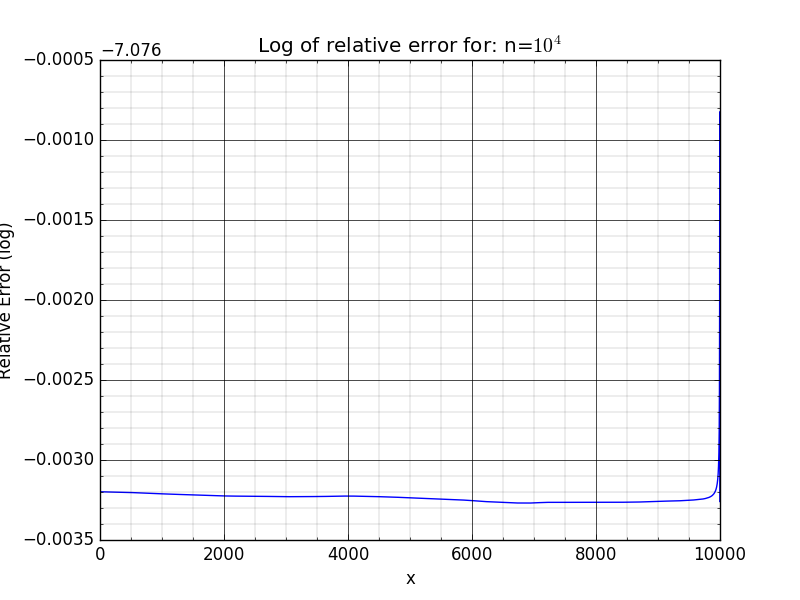
\includegraphics[scale=0.22]{4_error.png}
%\centering
%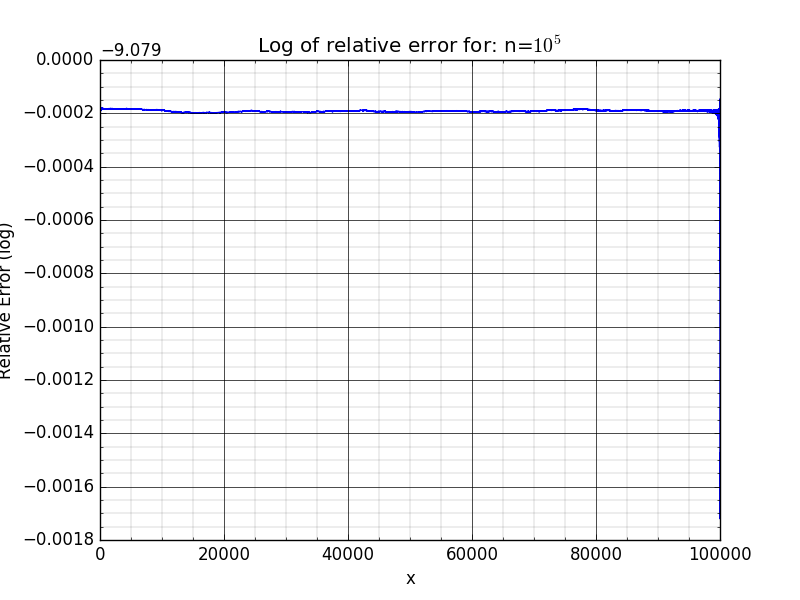
\includegraphics[scale=0.22]{5_error.png}\\
%\centering
%\caption{ Plots of the relative error between analytical and exact solution for numerical Gaussian elimination}
%\end{figure}
%
%Plots of the relative error between analytical and exact solution for numerical Gaussian elimination. Additionally, to verify that the algorithm was working correctly, the overall error as the solver progresses was captured and plotted since the variations in relative error can seem unintuitive. For each n, the average of the relative error is acquired. Additionally, to verify that the algorithm was working correctly, the overall error as the solver progresses was captured and plotted since the variations in relative error can seem unintuitive. For each n, the average of the relative error is acquired.\\
%
%\begin{figure}[H]
%	\centering
%	\graphicspath{ {c:/Users/charl/Documents/Precision/Gauss/}{C:/Users/Mike/Documents/GitHub/sayboltm/PHY480/Project1/Report/Precision/Gauss/}}
%	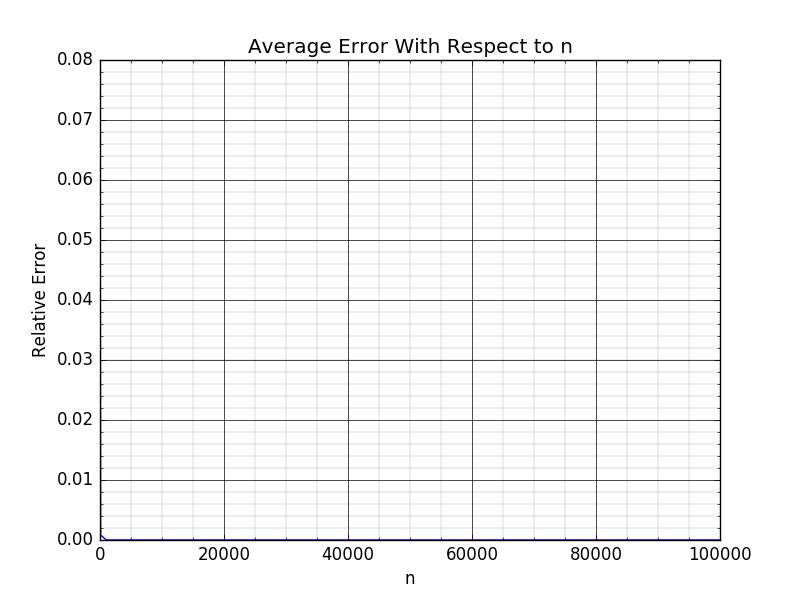
\includegraphics[scale=0.22]{BigError.png}
%	\caption{Average error with respect to n for Gaussian elimination on a linear scale}
%\end{figure}
% \pagebreak
%As n is increased, the overall relative error decreases, which is to be expected as the approximation is closer to the exact result. It is easier to see the trend when plotted on a log scale.\\
%
%\begin{figure}[H]
%\centering
%\graphicspath{ {c:/Users/charl/Documents/Precision/Gauss/}{C:/Users/Mike/Documents/GitHub/sayboltm/PHY480/Project1/Report/Precision/Gauss/}}
%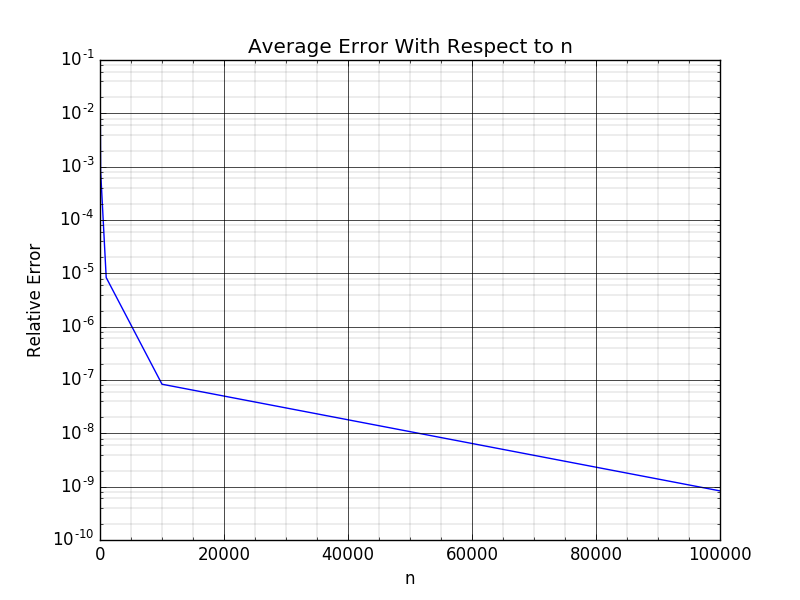
\includegraphics[scale=0.22]{BigError_log.png}
%\caption{Average error with respect to n for Gaussian elimination on a log scale}
%\end{figure}

\subsection{LU Decomposition:}
%Figure a shows the analytical solution and the numerical solution for various n using the LU decomposition function-based solver. As n increases, the result is more tightly fit to the analytical solution which is expected.\\
%
%\begin{figure}[H]
%\centering
%\graphicspath{ {c:/Users/charl/Documents/Precision/LU/}{C:/Users/Mike/Documents/GitHub/sayboltm/PHY480/Project1/Report/Precision/Gauss/}}
%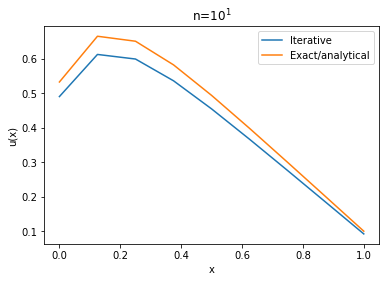
\includegraphics[scale=0.22]{1.png}
%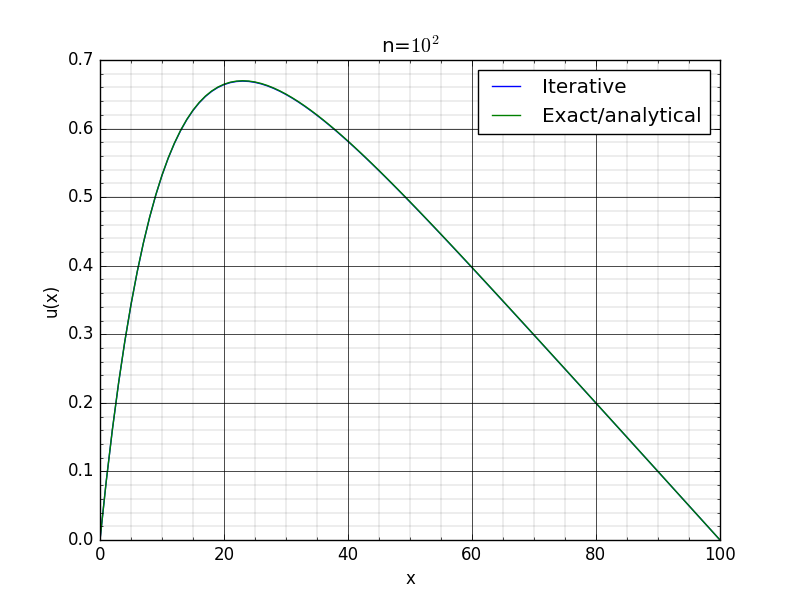
\includegraphics[scale=0.22]{2.png}
%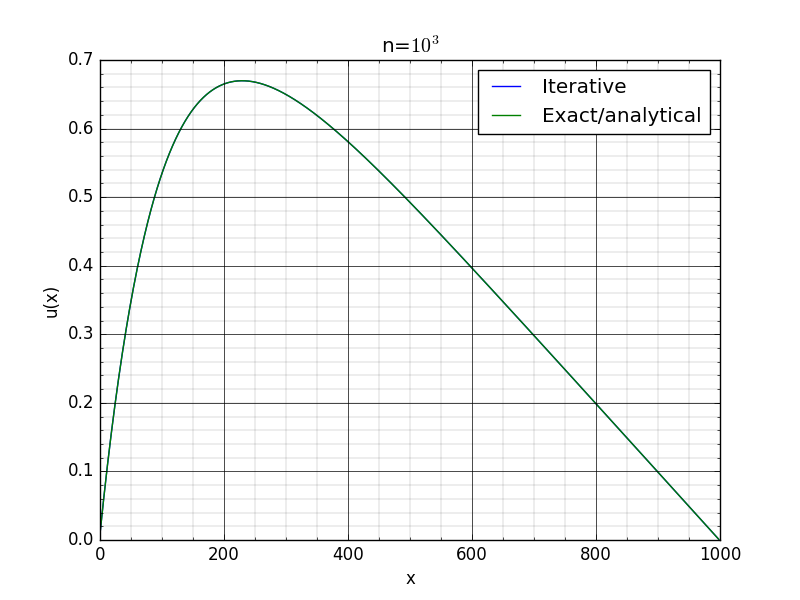
\includegraphics[scale=0.22]{3.png}
%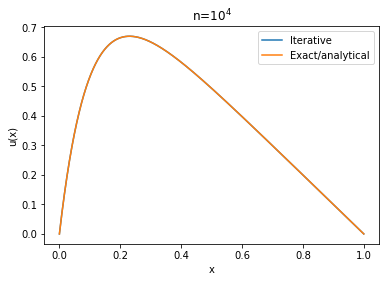
\includegraphics[scale=0.22]{4.png}\\
%\centering
%\caption{Plots of the analytical solution and numerical solution for solving with LU decomposition. The relative error is plotted for the LU decomposition as well in figure b.}
%\end{figure}
%
%\begin{figure}[H]
%\centering
%\graphicspath{ {c:/Users/charl/Documents/Precision/LU/}{C:/Users/Mike/Documents/GitHub/sayboltm/PHY480/Project1/Report/Precision/LU/}}
%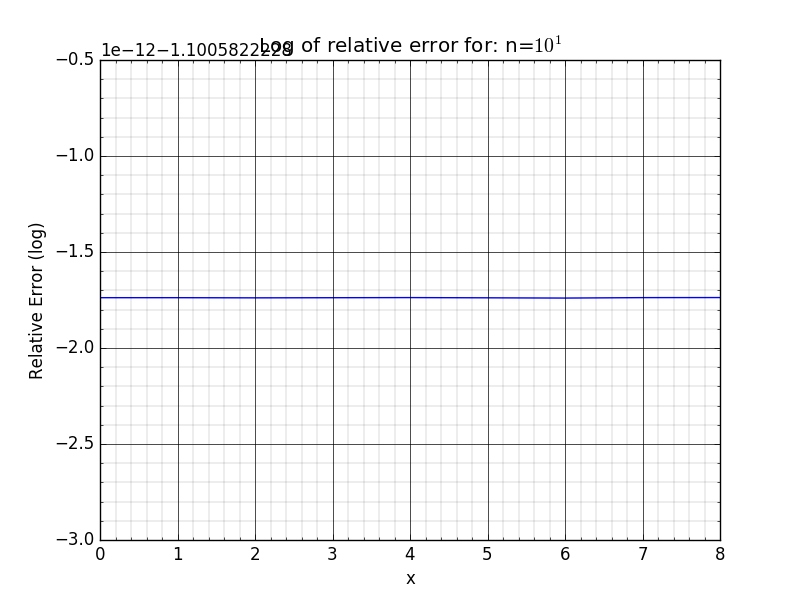
\includegraphics[scale=0.22]{1_error.png}
%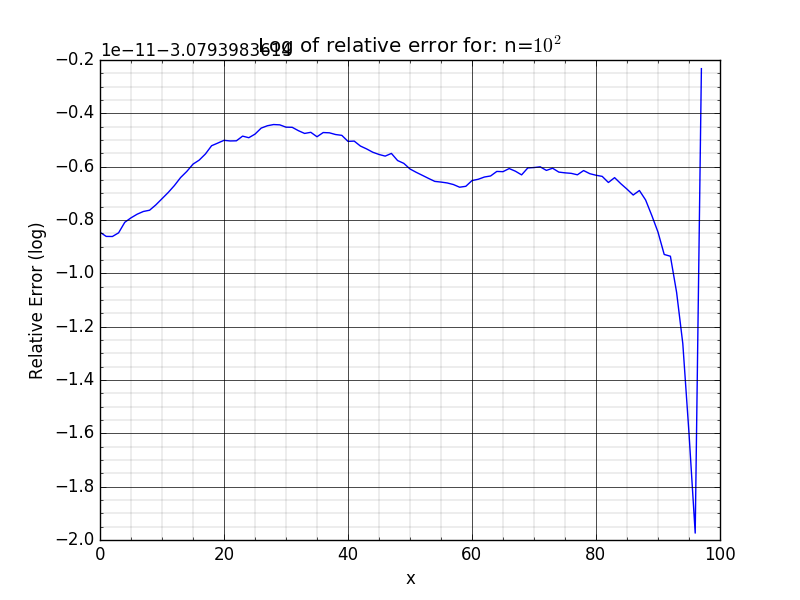
\includegraphics[scale=0.22]{2_error.png}
%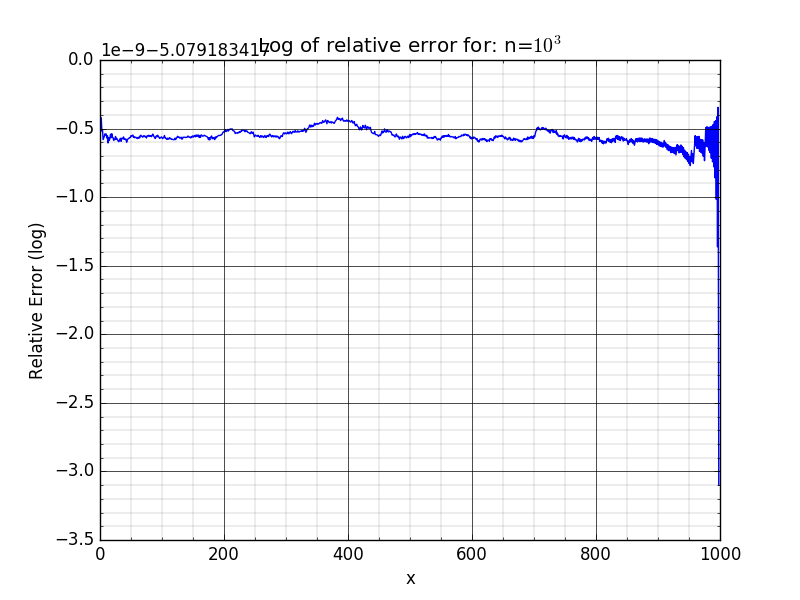
\includegraphics[scale=0.22]{3_error.png}
%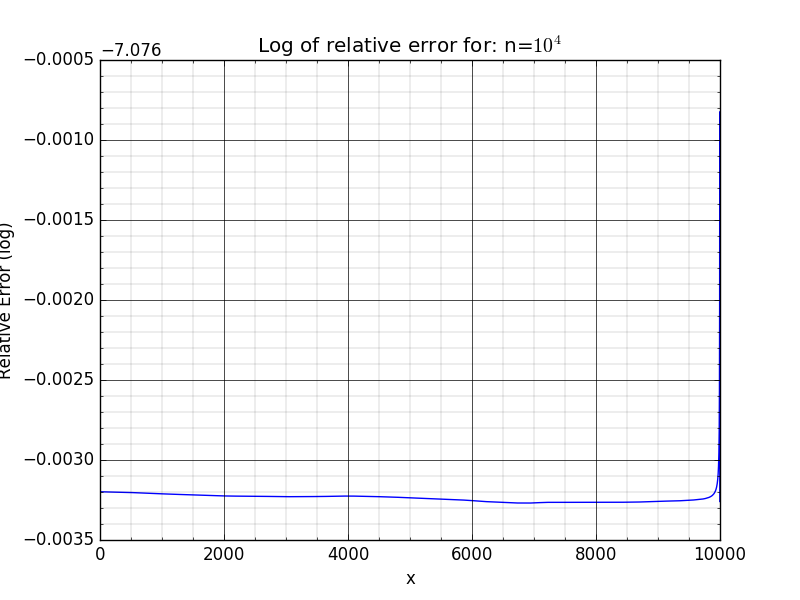
\includegraphics[scale=0.22]{4_error.png}\\
%\centering
%\caption{ Plots of the relative error between analytical and exact solution when solving with LU decomposition.	The overall error is also plotted, both on linear and log scales}
%\end{figure}
%
%\begin{figure}[H]
%\centering
%\graphicspath{ {c:/Users/charl/Documents/Precision/LU/}{C:/Users/Mike/Documents/GitHub/sayboltm/PHY480/Project1/Report/Precision/LU/}}
%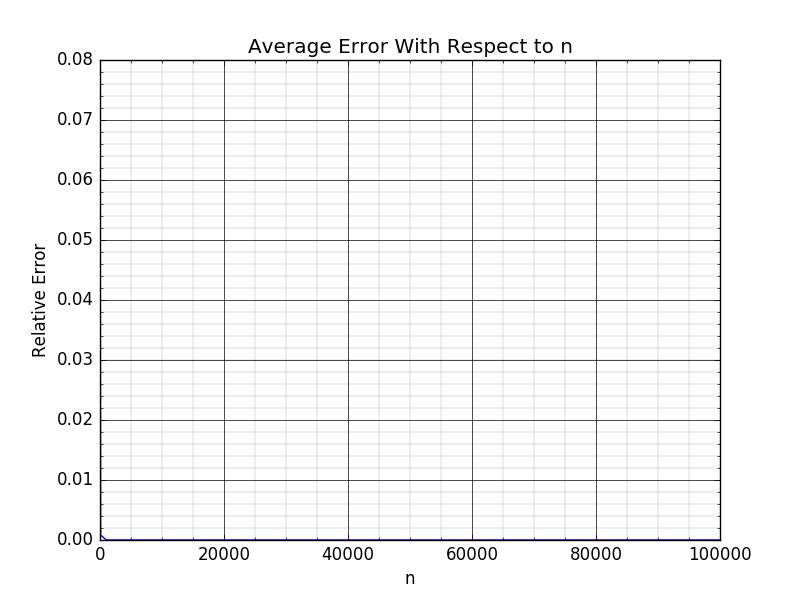
\includegraphics[scale=0.22]{BigError.png}
%\caption{Average error for LU decomposition on a linear scale}
%\end{figure}
%
%\begin{figure}[H]
%\centering
%\graphicspath{ {c:/Users/charl/Documents/Precision/LU/}{C:/Users/Mike/Documents/GitHub/sayboltm/PHY480/Project1/Report/Precision/LU/}}
%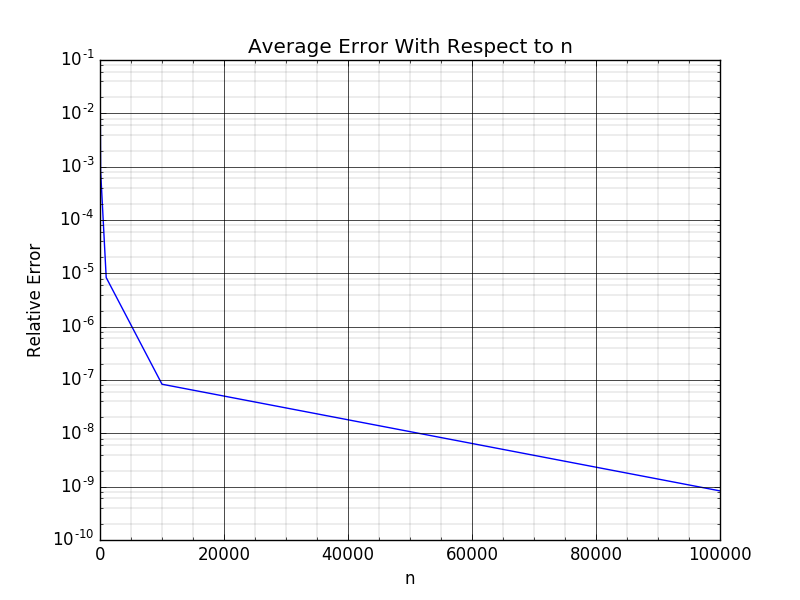
\includegraphics[scale=0.22]{BigError_log.png}
%\caption{Average error for LU decomposition on a log scale}
%\end{figure}
%
%Interestingly enough, the LU decomposition could only go to $n=10^4$ before running out of memory instead of $n=10^5$ for the Gaussian elimination solver. Perhaps the implementation in the $Numpy$ library does not allocate memory well.


\subsection{Speed of Execution}
%Each method that has been utilized to solve the original equation has been timed using the $date.now()$ functionality in Python. The fastest method was the General Gauss Elimination while LU Decomposition was lagging behind it. While I was definitely limited by my computing power I believe that these times could be reproduced by any other computer with reasonable computer power. The LU Decomposition was an average of 10 times slower than the General Solver.\\
%\begin{table}[H]
%	\centering
%	\bigskip
%	\bigskip
%	\bigskip
%	
%	\begin{tabular}{l|l|l|l|l|}
%		& n = 2    & n = 3    & n = 4    & n = 5    \\ \hline
%		LU Decomposition  & 0.001441 & 0.014482 & 0.12671  & 54.6002  \\ \hline
%		Gauss Elimination & 0.008974 & 0.063471 & 0.575171 & 5.686529 \\ \hline
%	\end{tabular}
%	\caption{This chart shows how the average time for each method}
%\end{table}
%The chart shows the average time for each method run ten (10) times. At $n < 5$ the LU Decomposition no longer is of the same magnitude, but it 10 times larger than the average times of the Gauss Elimination. 
%\pagebreak
%\section{Conclusions}
%From examining all of the methods used to solve the original linear equation we have concluded that the Gauss Elimination method is the most efficient at finding our solution, followed by the LU Decomposition. Lastly the least efficient method used to solve the linear equation was the LU Decomposition Solver.
%\section{References}
%\begin{itemize}
%	\item  Hjort-Jensen, M., 2015. Computational physics. \\$https://github.com/CompPhysics/ComputationalPhysics/$
%\end{itemize}

\end{document}
